\chapter{Byudvikling}
Dette kapitel handler om byudvikling i Aalborg. I kapitlet bliver Aalborgs udvikling fra en købsstad til en industriby til en kompetenceby beskrevet. Kommuneplaner generelt og  Aalborgs kommuneplan bliver beskrevet, hvor der bliver lagt særligt fokus på Vækstaksen. Lokalplanen for området hvor Strøybergs Palæ står bliver også beskrevet.

\section{Aalborgs udvikling til kompetence by}
Aalborg har i de seneste årtier været under stor udvikling fra at være en industriby, til at blive en videns- og uddannelses by.  Gamle industriområder, som en gang kendetegnede Aalborg, bliver i dag omdannet til nye boliger, kontorer, kultur og uddannelsessteder.

Byen Aalborg blev grundlagt tilbage i vikingetiden. Området var attraktivt da det havde gode havnemuligheder ud til Limfjorden. Byen blev i begyndelsen primært brugt som midtpunkt for markedspladser og værksteder. På grund af dette, var det ikke stor udvikling i byen, idet byen kun blev brugt som en form for samlingssted og ikke fast bosættelse. Det vides ikke sikkert hvornår Aalborg fik tildelt købstadsrettigheder men man ved, at byen begyndte at udvikle sig kraftigt fra ca. 1350 og frem. Dvs. at det højst sandsynligt er omkring denne periode, at byen fik tildelt købstadsrettigheder. Byens primære økonomi lå i salget af sild og korn. I 1600-tallet havde Aalborg stort set monopol på korneksport fra hele Vendsyssel og omkring Limfjorden. Byens købmænd tjente især stort på eksport til Norge og Tyskland.

I 1700-tallet oplevede Aalborg et fald i salget. Byen var stadig blandt de største i Danmark, men sildefiskeriet og korneksporten var ikke lige så attraktivt, som det havde været. Dette blev forværret med tabet af Norge i 1814, hvilket medførte at byen mistede vigtige handelsmarkeder.

På dette tidspunkt ligger Aalborg på sit laveste i en længere periode. I 1830’erne blev der etableret nye industrivirksomheder (heriblandt forløberen til De Danske Spritfabrikker), som var med til at opveje de økonomiske tab. Dette er således begyndelsen på Aalborgs bevægelse hen imod at blive en industriby, som i slutningen af 1800-tallet for alvor tog fat, som konsekvens af industrialiseringen, som bredte sig i hele Danmark i denne periode. Det var med udviklingen af dampmaskinen, at den industrielle revolution tog fat. Aalborg blev hjemsted for mange store virksomheder, specielt cementfabrikker, heriblandt Aalborg Portland, som nød godt af de store mængder kridt i Aalborgs undergrund og den nærliggende havn for transport. Disse industrivirksomheder satte for alvor gang i den industrielle udvikling i byen og medførte, at Aalborg gennem 1900-tallet var en udpræget arbejderby. Byen blev kendt som ”byen med de rygende skorstene”. 

Aalborg er i dag under omdannelse fra at være industriby til at være en kompetenceby. Siden 1960’erne og -70’erne, da henholdsvis Aalborg Seminarium og Aalborg Universitet blev grundlagt, har industrivirksomheder haft dalende betydning for byen. I slutningen af 1990’erne ombyggede man mange gamle industriområder til kontorer og boliger, pga. et stigende behov for dette. Ved år 2000 var op mod 60 procent beskæftiget inden for service- og uddannelseserhverv. På dette tidspunkt var det kun de mest veletablerede industrivirksomheder, som blev stående, mens mindre industrivirksomheder flyttede væk. Ved slutningen af 00’erne ses den største udvikling i form ombygningen af havnefronten øst for Limfjordsbroen, Kraftværket Nordkrafts omdannelse til kulturbygning og et stigende antal ungdomsboliger. I 2014 lukkede De Danske Spritfabrikker efter at være solgt til et Norsk selskab, som flyttede produktionen til Norge. Bygningen som nu står tilbage, skal efter planerne, omdannes til en international kunst- og kulturby.


\section{Kommuneplaner og Aalborgs kommuneplan}
En kommuneplan, er en kommunes overordnede plan for kommunens fremadrettede udvikling inden for de næste 12 år. Alle Danmarks kommuner har pr. lov, krav på, at have en kommuneplan. Det er kommunernes byråd, som står for at lave kommuneplaner. Kommuneplaner handler om hvordan erhverv, boliger og diverse servicefunktioner skal placeres i forhold til hinanden. En kommuneplan skal også vise en kommunes plan for trafikaflastning, det åbne land, skov områder, grønne områder mm. Byrådene, som laver kommunaplanerne, kan ikke gøre lige præcis som de vil, planerne skal overholde planloven. Kommuneplanerne er ikke direkte bindende for borgerne i kommunerne, f.eks. er grundejere ikke forpligtede til at overholde planen, dog siger planlovens §12, stk. 1, at kommunalbestyrelsen har pligt til at forsøge at få kommuneplanen gennemført. En kommuneplan indeholder følgende:

\begin{description}
\item [Hovedstruktur] er den overordnede, strategiske og sammenfattende fysiske plan for kommunen. Hovedstrukturen fastlægger de overordnede mål for udviklingen indenfor de enkelte områder og kommunen.
\item [Retningslinjer] udgør rammerne for kommuneplanen og kommunens administration af planlovens landzonebestemmelser og anden lovgivning indenfor bygge-, natur- og miljølovgivning.
\item [Kommuneplanrammer] styrer den overordnede anvendelse af kommunens arealer og danner rammer for indholdet af nye lokalpaner. Rammedelen er bygget op af bybeskrivelser, der beskriver udviklingen i kommunens byer og bydele, samt andre geografiske områder. Borgerne i kommunerne skal ikke direkte overholde kommuneplanrammerne, men de skal overholde de lokalplaner som bliver lavet ud fra kommuneplanrammerne.
\item [Bilag og tilhørende planredegørelse] beskriver forudsætningerne for ændringer i den konkrete planlægning. 
\end{description}

\subsection{Vækstaksen som byens motor}
Aalborgs fremadrettede udvikling skal være en målrettet og fokuseret byvækst, som skal ske i en vækstakse som strækker sig fra lufthavnen i nordvest til havnen i øst. Vækstaksen er vist på Figur \ref{fig:Vaekstakse1}

\begin{figure}[H] 
\centering
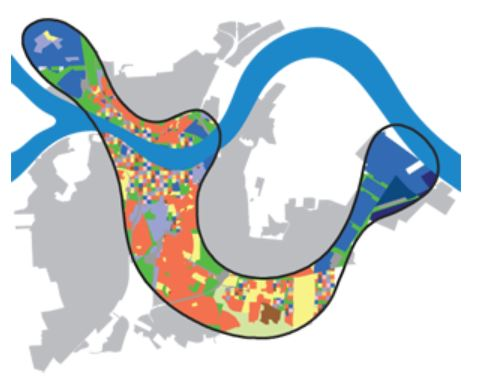
\includegraphics[width=0.50\textwidth]{billeder/Vaekstakse1}
\caption{Figuren viser den vækstakse som Aalborg primært skal udvikle sig i.}
\label{fig:Vaekstakse1}
\end{figure}

Kommunen vil have en koncentreret udvikling i denne vækstakse, hvilket betyder at offentlige og private investeringer skal koncentreres i vækstaksen, så synergier opstår og byen styrkes i fremtiden. I vækstasken skal der være tilbud og plads til alle behov og aldersgrupper, med hensyn til bolig, transport, natur, indkøb og fritidsinteresser. Vækstaksens endepunkter ved lufthavnen i nordvest og ved havnen i sydøst, skal udvikles som attraktive trafikbaserede erhversområder med gode forbindelser til resten af verden. Vækstaksen skal opnå storbykarakter, som kan tiltrække turister og fastholde både studerende og vidensarbejdere fra både ind- og udland. Det er vigtigt for vækstaksen at havnefronten, Karolinelund, Godsbanearealet, Eternitten, det østlige Aalborg, de bynære erhversarealer mm. skal færdiggøres og videreudvikles, da det skal sikre momentum og skabe attraktive og bæredygtige levevilkår

På Figur \ref{fig:Vaekstakse2}  er de udviklingsområder i vækstaksen med store potentialer for yderligere udvikling af Aalborg markeret. De markarede områder kan bidrage til udvikling af byen i form af boliger, arbejdspladser og styrkede grønne arealer. Nem og hurtig tilgængelighed i vækstaksen ligger til grund for udviklingen, idet målet med udviklingen er en styrket, bæredygtig udvikling kombineret med øget fremkommelighed.

\begin{figure}[H]
\centering
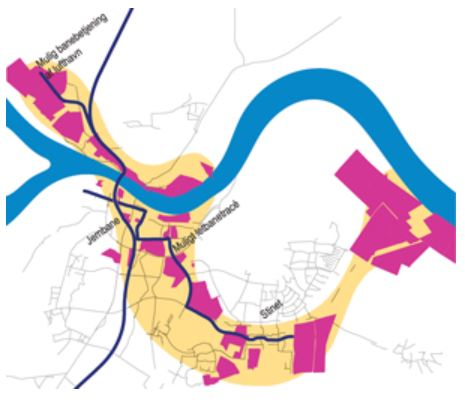
\includegraphics[width=0.50\textwidth]{billeder/Vaekstakse2}
\caption{Figuren viser de områder (markeret med lilla) som Aalborg Kommune primært vil have at Aalborg udvikler sig omkring.}
\label{fig:Vaekstakse2}
\end{figure}

Mobilitet er rygraden i vækstaksen, hvilket betyder, at det skal være let og hurtig adgang mellem centrale funktioner som f.eks. rekreative områder. Områderne omkring  knudepunkterne, vist på Figur \ref{fig:Vaekstakse3}, skal i særlig grad fortættes. Der skal sikres meget gode muligheder for at skifte mellem diverse transportformer, indkøb, service og bosætning, samt adgangsforholdene til knudepunkterne skal styrkes. Der skal på samme tid være en sammenhæng mellem vækstaksens vestlige og østlige endepunkter og byens centrum. 

\begin{figure}[H] 
\centering
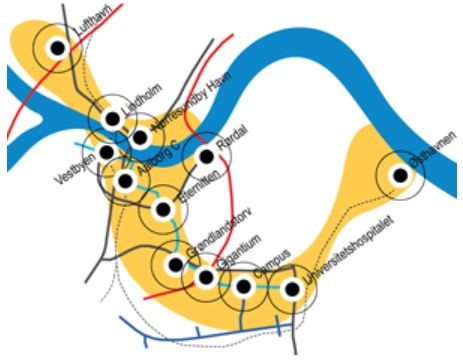
\includegraphics[width=0.50\textwidth]{billeder/Vaekstakse3}
\caption{Figuren viser de knudepunkter i Aalborgs vækstakse som der primært skal fortættes omkring. Infrastrukturen skal være særlig god i disse knudepunkter.}
\label{fig:Vaekstakse3}
\end{figure}

Kompetencebyen i Aalborg skal videreudvikles, dette gøres ved, at uddannelsesinsitutioner og ungdomsbolier koncentreres i vækstaksen. De mange studerende er med til at skabe liv i byen og hjælper med at lave en særlig oplevelseszone i centrum af Aalborg. Vækstaksen skal hjælpe Aalborg med at skabe et internationalt præg, som kan tiltrække udenlandske forskere, studerende og vidensarbejdere. Aalborgs Universitets Campus i Aalborg Øst skal udvikles til et regionalt midtpunkt med et meget levende studiemiljø og med diverse vidensvirksomheder.


\begin{figure}[H] 
\centering

\includegraphics[width=0.50\textwidth]{billeder/Vaekstakse4}
\caption{Figuren viser de områder i Aalborgs vækstakse hvor der i særlig grad er og skal bygges ungdomsboliger, uddannelsesinstitutioner og vidensvirksomheder}
\label{fig:Vaekstakse4}
\end{figure}



\subsection{Byudviklingsprincipper for Aalborg}
Et af hoved byudviklingsprincipperne for Aalborgs kommuneplan er, at byen først og fremmest skal udvikles indenfor de eksisterende grænser, ved hjælp af fortætning og byomdannelse. Denne udvikling skal så være koncentreret særligt i vækstaksen. Sammen med fortætningen af byen skal der også udvikles en række grønne nærområder, så byen opnår en høj levekvalitet. Det er vigtigt for Aalborg, at byudviklingen tager hensyn til fjorden og landskabet ved Aalborg. På Figur \ref{fig:Byudviklingsprincipper1} ses byudviklingsprincipperne for vækstaksen.

\begin{figure}[H] 
\centering
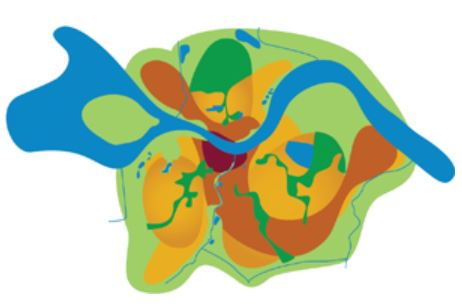
\includegraphics[width=0.50\textwidth]{billeder/Byudviklingsprincipper1}
\caption{Figuren viser Aalborg Kommunes vision for Aalborg.}
\label{fig:Byudviklingsprincipper1}
\end{figure}

I Aalborgs kommuneplan bliver der også lagt stor vægt på at sikre byen mod klimaændringer i fremtiden. I fremtiden forventes der mere nedbør og at vandstanden i havene stiger. Da fjorden løber igennem Aalborg, er Aalborg særligt udsat for fremtidige oversvømmelser. I klimastrategien betyder dette, at ved alt byggeri under kote 2,5m foretages der en klimasikring. Aalborg Kommune vil udarbejde en klimatilpasningsplan for hele kommunen, som skal være baseret på en kortlægning af oversvømmelsesrisici. For yderligere at sikre byen mod fremtidiger oversvømmelser, skal byen som udgangspunkt ikke udvikle sig længere mod de lavtliggende områder. Aalborg Kommune sigter efter at anvende de forøgede vandmængder rekreativt i byen. På Figur \ref{fig:Byudviklingsprincipper2} ses worst-case scenario for oversvømmelse i Aalborg-området 

\begin{figure}[H] 
\centering
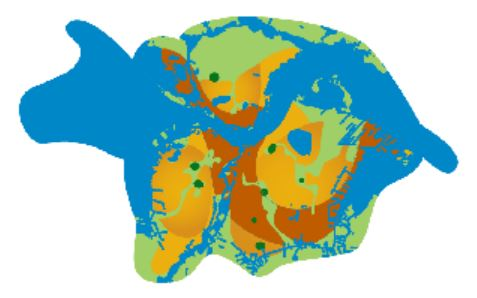
\includegraphics[width=0.50\textwidth]{billeder/Byudviklingsprincipper2}
\caption{Figuren viser worst-case scenario for oversvømmelse i Aalborg, når fjordens vandstand stiger.}
\label{fig:Byudviklingsprincipper2}
\end{figure}

Mobilitet skal ligge til grund for byens fremtidige udvikling, hvor især de bløde trafikanter skal prioriteres i midtbyen. I Aalborg skal der være stort fokus på bæredygtigt transport. Vækstaksen skal medvirke til at skabe et behov for en letbaneforbindelse, der skal bygges en tredje Limfjordsforbindelse og opføres en paralleltunnel. Der skal også laves en banebetjening til lufthavnen. På Figur \ref{fig:Byudviklingsprincipper3} ses mobilitetsplanen for Aalborg.

\begin{figure}[H] 
\centering
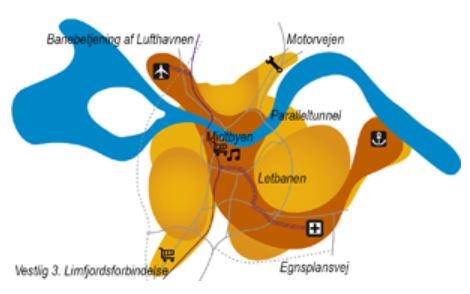
\includegraphics[width=0.50\textwidth]{billeder/Byudviklingsprincipper3}
\caption{Figuren viser Aalborg Kommunes mobilitetsplan for Aalborg, hvor blandt andet en letbaneforbindelse og en 3. limfjordsforbindelse indgår.}
\label{fig:Byudviklingsprincipper3}
\end{figure}

I perioden 2012-2024 viser Aalborg Kommunes befolkningsprognose, at der kommer en tilvækst på cirka 7000 borgere i Aalborg. Behovet for nye boligere ligger derfor, i følge Aalborg Kommune, på 6-7000, grundet faldende husstandsstørrelser. Indenfor det planlagte område vurderes det, at der er plads til cirka 8000 boliger, disse boliger skal primært skabes ved at omdanne eksisterende byområder til tættere byområder. Som nævnt tidligere, skal Aalborg primært udvikles på de højtliggende områder, Figur \ref{fig:Byudviklingsprincipper4} illustrerer området, som Aalborg skal udvikle sig på.


\begin{figure}[H] 
\centering
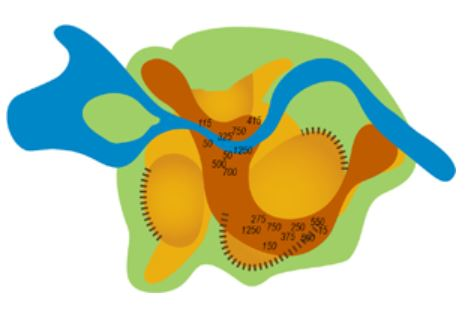
\includegraphics[width=0.50\textwidth]{billeder/Byudviklingsprincipper4}
\caption{Figuren viser det område hvor Aalborg skal udvikle sig på, i følge kommuneplanen.}
\label{fig:Byudviklingsprincipper4}
\end{figure}


Det er vigtigt, at Aalborg i fremtiden udvikler sig til at blive en blå by (en by med mange søer og vandløb). Der skal etableres en blå ring rundt om byen, bestående af en række søer og vandløb, ikke kun pga. rekreative årsager, men også funktionelle årsager, da søerne og vandløbene kan aflede en del af de vandmasser, som vil komme i fremtiden. Søerne skal etableres i tidligere råstofgrave, som ligger rundt om Aalborg. Figur \ref{fig:Byudviklingsprincipper5} viser Aalborg som en blå by.

\begin{figure}[H] 
\centering
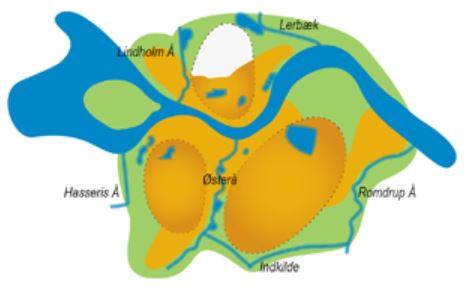
\includegraphics[width=0.50\textwidth]{billeder/Byudviklingsprincipper5}
\caption{Figuren viser Aalborg Kommunes vision af Aalborg som en blå by}
\label{fig:Byudviklingsprincipper5}
\end{figure}

Aalborg skal ikke kun være en blå by, det skal også være en grøn by. Der skal etableres en grøn ring rundt om byen og på bakkerne, langs fjorden og i Østerådalen skal der laves en række grønne forbindelser. Aalborgs markante bakketoppe skal i fremtiden fremstå som skovklædte kendetegn. Figur \ref{fig:Byudviklingsprincipper6} viser Aalborg Kommunes vision af Aalborg som en grøn by.

\begin{figure}[H] 
\centering
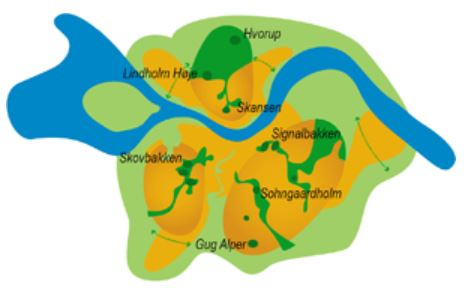
\includegraphics[width=0.50\textwidth]{billeder/Byudviklingsprincipper6}
\caption{Figuren viser Aalborg Kommunes vision af Aalborg som en grøn by}
\label{fig:Byudviklingsprincipper6}
\end{figure}


\subsection{Fokus på bykvalitet}
I Aalborg skal der være stort fokus på god bykvalitet, som er afhængig af stedet. Det er vigtigt, at velfungerende bygninger og byrum udvikles på baggrund af stedets særlige kvaliteter og potentialer, byens rum skal udvikles til at blive attraktive og rare at opholde sig i. Konkrete mål for bykvalitet er forskelligt fra nærmiljø til nærmiljø. Arkitektonisk kvalitet og kulturhisotrie skaber en identitet til nærmiljøerne og dette skal sikres. Byens kvaliteter skal være forskellige så der er noget for både beboere, studerende, kunder, turister og arbejdere.

\begin{figure}[H] 
\centering
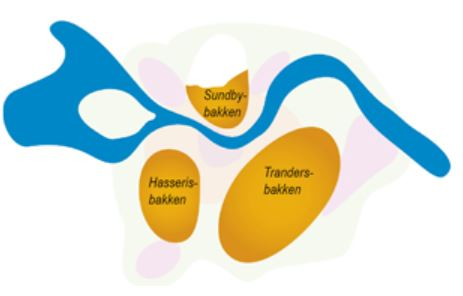
\includegraphics[width=0.50\textwidth]{billeder/Bykvalitet1}
\caption{Figuren viser Aalborgs tre store bakkeområder, Hasseri-, Sundby- og Trandersbakken.}
\label{fig:Bykvalitet1}
\end{figure}

Aalborg er en bakkeby og dette skal tydeligt kunne ses på byen. Landskab, udsigt, lys og luft er nogle særlige kvaliteter, som skal fremmes ved Aalborgs tre store bakker. På Figur \ref{fig:Bykvalitet1} ses Aalborgs tre store bakkeområder. Det er vigtigt, at bebyggelsen giver plads til naturen. Aalborgs forskellige forstadsområder skal udvikles, som veldefinerede nærmiljøer med lokal identitet og særpræg. Udviklingen af forstadsområderne skal blandt andet ske ved at oprette en række gode mødesteder, en forbedret infrastruktur, nye boligformer og ved nye multifunktionelle bygninger og byrum, som skal skabe liv. Fremtidige forstadsområder skal udvikles mere bæredygtigt, blandt andet ved at gå væk fra enfamiliehuse, da dette vil åbne op for større naturområder og mindre behov for biler.

\begin{figure}[H] 
\centering
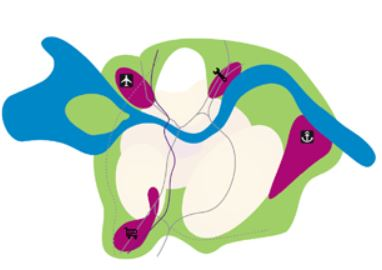
\includegraphics[width=0.50\textwidth]{billeder/Bykvalitet2}
\caption{På figuren er Aalborgs primærer erhversområder markeret med lilla.}
\label{fig:Bykvalitet2}
\end{figure}

Aalborg skal i fremtiden have fire veldefinerede erhvervsområder, lufthavnsområdet, City Syd, Aalborg Havn og Nørre Uttrup, områderne kan ses på Figur \ref{fig:Bykvalitet2}. De fire erhvervsområder skal have en høj funktionalitet, de skal være nemt tilgængelige og der skal være gode muligheder for transport af varer til og fra dem. City Syd skal i fremtiden være karakteriseret af storskalashopping. Området skal derved fungere, som et supplement til midtbyen. Aalborg Havn og lufthavnsområdet skal sikres fremtidige udviklingsmuligheder. 

\subsection{Nødvendige forbindelser - mobilitet}
I fremtiden skal en væsentlig større del af trafikken i Aalborg foregå med bæredygtige transportformer. I bymidten skal fodgængere, cyklister og kollektiv trafik prioriteres over biler. Et cykelstinet af høj kvalitet skal sikre cyklisterne meget høj tilgængelighed i Aalborg. Det skal være nemt og enkelt at tage fra midtbyen til universitetet, universitetshospitalet, Østhavnen og lufthavnen. Nye parkeringspladser i midtbyen skal begrænses, og i stedet opføres i store P-huse eller P-kældre langs randgaderne. På Figur \ref{fig:Mobilitet1} ses de veje, som primært skal aflaste trafikken i vækstakse området.

\begin{figure}[H] 
\centering
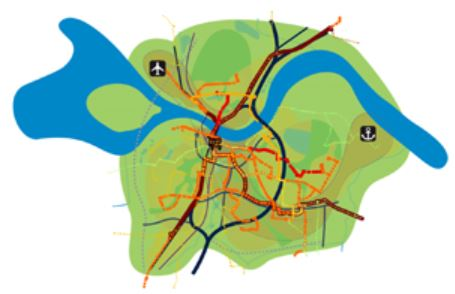
\includegraphics[width=0.50\textwidth]{billeder/Mobilitet1}
\caption{Figuren viser de veje der primært skal aflaste trafikken i vækstakse området.}
\label{fig:Mobilitet1}
\end{figure}

\subsection{Opsamlende analyse}
Aalborgs Kommunes kommuneplan ligger stort fokus på, at Aalborg skal udvikle sig bæredygtigt både for miljøet og for menneskerne i byen. Kommuneplanen ligger stort fokus på bæredygtigt transport, hvor de vil have bilerne ud af centrum og i stedet for have busser, cyklister, fodgængere og en letbane ind i centrum. Letbanen bliver ikke til noget, da det ikke var muligt at få statslig støtte til projektet, hvilket er et stort tilbageslag for Aalborg Kommunes vision for Aalborg, da letbanen skulle bidrage markant til den bæredygtige transport. I stedet for en letbane har kommunen etableret en del af en busvej, som efter planen skal starte ved Aalborg Busterminal og slutte ved Aalborg Universitet og med en fremtidig endestation ved nybyggeriet Aalborgs Universitetshospital. Busvejen skal gå igennem Øgadekvarteret, Vejgaard, under motorvejen og forbi Gigantium. Aalborg Kommunes plan om at få borgerne til at droppe bilerne til fordel for offentlig transport, bliver svært da det ofte kan føre til længere transport tider og nogle gange også være dyrere. Andre grunde til at det kan være svært for kommunen at få folk til at skifte fra bil til offentlig transport er f.eks. kultur, vaner og frihedsfølelsen ved at køre en bil man ejer. Mange vælger offentlig transport fra, men nogle vælger cyklen til. En af grundene til dette kan være Aalborg Kommunes store fokus på at lave et godt cykelstinet. Aalborg Kommune vil have en fortætning af byen omkring en række knudepunkter, se Figur \ref{fig:Vaekstakse3}, langs vækstaksen. Ved disse knudepunkter vil kommunen have en høj mobilitet med mulighed for at skifte mellem diverse transportformer, dette kan være et problem da en fortætning af byen, kan give mangel på plads til f.eks. parkeringspladser. En løsning på dette vil være etablering af en række P-kældere, hvilket igen bliver et problem, da disse er relativt dyre. Kommunens plan om at adskille by og tunge erhversområder er meget godt for bymilljøet og erhvervet. Det er godt for erhvervsområderne på den måde, at det markant nedsætter transporttiden, da lasten ikke skal igennem byen først, men derimod bare kan transporteres direkte videre med skib og lastbil. Det gode for bymiljøet er, at der kommer færre lastbiler igennem byen, som både forurener meget og forsinker trafikken. Kommunens plan om et etablere en tredje Limfjordsforbindelse og en paralleltunnel er i følge en VVM-undersøgelse en meget god samfundsinvestering som vil spare samfundet for en stor mængde rejsetimer og penge.

Aalborg Kommune er en kommune, som i lang tid har haft fokus på bæredygtighed, hvilket blandt andet kan ses på Aalborgs Bæredygtighedsfestival. Dette kan også ses i Aalborgs Kommunes kommuneplan, hvor der bliver lagt fokus på, at Aalborg skal være en blå og grøn storby, hvor der blandt andet skal være en række søer, vandløb og grønne områder i og omkring Aalborg. Det er ikke tilfældigt at Aalborg Kommune ligger stort fokus på at udvikle kommunen bæredygtigt. Nogle af grundene hertil er, at det er "in" at være og tænke bæredygtigt, mange borgere går op i bæredygtighed også ligger der en masse lovgivning til grund for dette, blandt andet planloven, som blandt andet kræver at kommunerne udarbejder strategiredegørelser for blandt andet "mindskelse af miljøbelastning" og "fremme af en bæredygtig byudvikling og byomdannelse", dette kaldes også "Agenda 21". Søerne der skal laves omkring Aalborg er ikke kun til rekreativt brug. Et eksempel på en af søerne som ikke skal bruges rekreativt er, søen som er blevet dannet i Aalborg Portlands kridtgrav, den skal bruges til at køle det kommende supersygehus. Etablering af diverse nye vandløb, søer og grønne området inde i centrum af Aalborg, kan give problemer, da kommunen på samme tid vil have at der sker en fortætning af byen. Pladsmangel vil højst sandsynligt føre til at, færre søer, vandløb og grønne områder bliver etableret i centrum. 

I kommuneplanen fremgår det at de tre store bakkeområdet Hasseri-, Sundby- og Trandersbakken, skal være præget af landskab, udsigt, lys og luft, hvilket betyder at der skal være grønne og åbne områder på bakkerne. Et andet sted i kommuneplanen står der at fremtidig byudvikling og byfortætning primært skal ske i disse områder, grundet stigende vandstande i fremtiden. For at dette kan lade sig gøre vil kommunen have at områder skal bestå af nye boligformer og gå væk fra de traditionelle enfamiliehuse.



\section{Lokalplan - Strøybergs Palæ}
En lokalplan bruges til at fastlægge bestemmelser for udviklingen af et område, som i dette tilfælde er Strøybergs Palæ. Lokalplanen skal være med til at give et overblik over området, samt være en plan over for hvordan området skal bruges og hvad der skal overholdes. Med en lokalplan sikrer man, at alle er enige om områdets udvikling og at bevaringsværdige bygninger bliver bevaret efter planloven. 

\begin{figure}[H] 
\centering
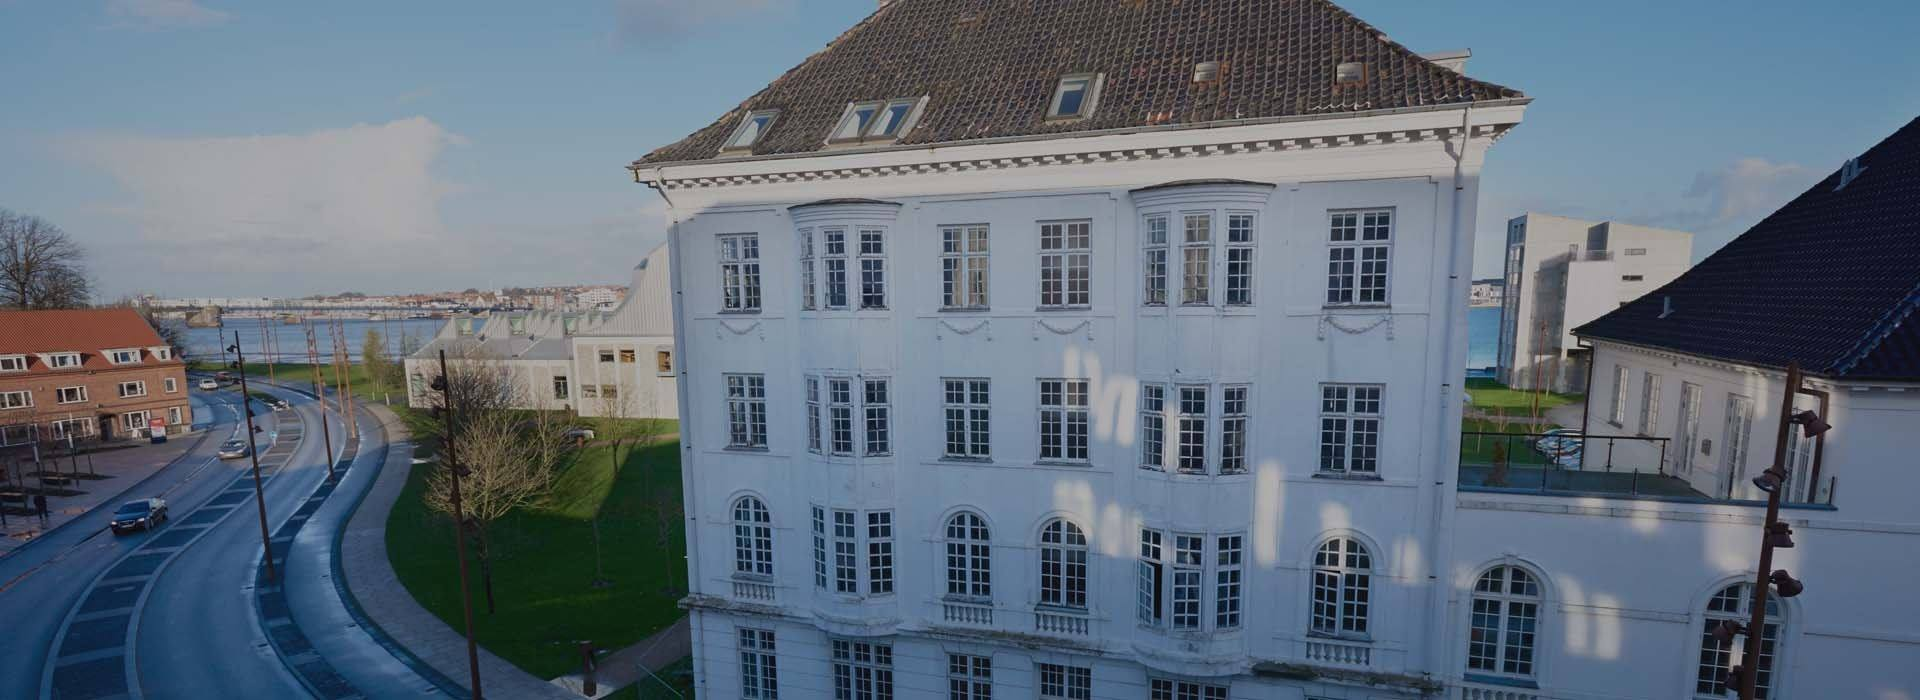
\includegraphics[width=0.50\textwidth]{billeder/Lokalplan3}
\caption{Strøybergs Palæ}
\label{fig:Lokalplan3}
\end{figure}



Den 12. november 2012 blev en ny lokalplan for Strøybergs Palæ vedtaget af Aalborg byråd (1-1-107 Strøybergs Palæ). I lokalplanen blev der fremlagt et forslag om at lave en tilbygning til hovedbygningen. Tilbygningen til Strøybergs Palæ skal bygges inden for lokalplanens fastlagte rammer. I dette afsnit gennemgås lokalplanen for Strøybergs Palæ, efter hvad der har relevans for opførelsen af en tilbygning. 

\begin{figure}[H] 
\centering
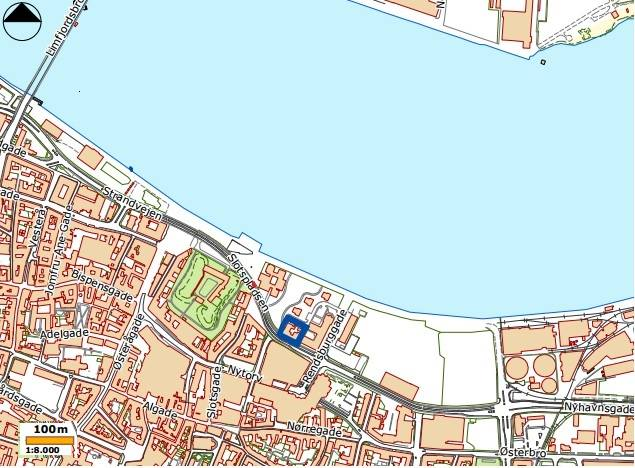
\includegraphics[width=0.50\textwidth]{billeder/Lokalplan1}
\caption{Kort over Aalborg Havnefront med Strøyberg Palæs lokalplanområde markeret med blåt}
\label{fig:Lokalplan1}
\end{figure}

Lokalplanen udgør et område, med et areal på 1200$ m^{2} $. Området ligger i tilknytning til havnefronten, ca. 100m fra Limfjorden, se Figur \ref{fig:Lokalplan1} . Strøybergs Palæ anvendes primært som en kontorbygning. Området er delt op i to dele, delområde A og B, se Figur \ref{fig:Lokalplan2}. Delområde A er den bevaringsværdige hovedbygning og delområde B er den bevaringsværdige sidebygning. Begge delområderne er kategoriseret til at have en bevaringsværdi på middel. Dvs. ved eventuel ombygning af bygningerne, skal der tages hensyn til det oprindelige udseende af bygningen. Tilbygninger og nybyggeri skal tilpasses det bevaringsværdige, men må stadig gerne udtrykke noget nutidigt design.



\begin{figure}[H] 
\centering
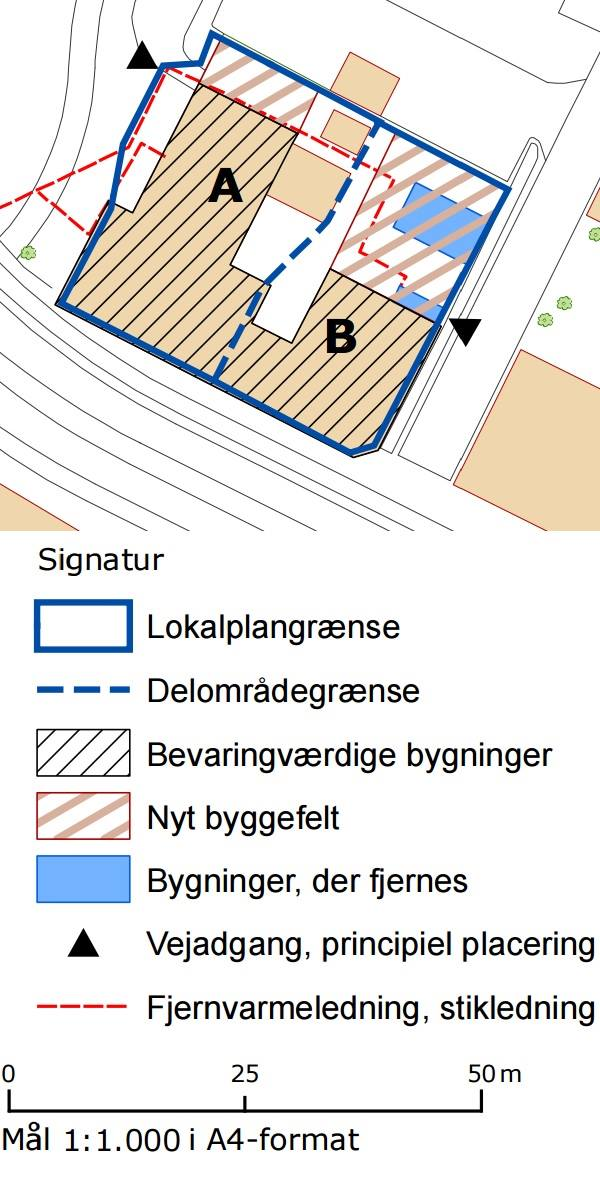
\includegraphics[width=0.50\textwidth]{billeder/Lokalplan2}
\caption{På denne figur ses delområde A og B, samt byggefeltet inden for lokalplanområdet, hvor tilbygningen kan være}
\label{fig:Lokalplan2}
\end{figure}

I Lokalplanen har man opstillet restriktioner for tilbygningen. Nedenfor vil de mest hovedsagelige blive gennemgået.

Tilbygningen skal bygges inden for byggefeltet illustreret på Figur \ref{fig:Lokalplan2}. Dette kræver, at mindre bygninger på området, som ikke er bevaringsværdige, nedrives til fordel for tilbygningen. Der er fastlagt for det samlede byggeareal i delområde A, at der maksimalt må være en bebyggelsesprocent på 350 procent. For delområde B er bebyggelsesprocenten maks. 320 procent. 

Strøybergs Palæ, som bygningen står nu, er op til 4½ etager og har en højde på ca. 22 meter. Dvs. 3 etager, 1 kælder og en tagetage. For den nye bebyggelse kan der bygges samme antal etager samt en tagetage, dog må den maksimale højde ikke overskride 19 meter. Med denne højde menes det ikke at have nogen effekt på udsigten til kysten, idet der er opført tre punkthuse med op til 7 etager, mellem lokalplanområdet og Limfjorden. Der kan være mulighed for at bygge kælderarealer til parkering, depot, teknik og lignende. Hvis der vælges at bygge en kælderetage, må der maksimalt være en lofthøjde på 2 meter over terræn ved område B, og 1.25 meter for område A. På grund af fremtidige vandstandsstigninger, skal kælderetagen desuden sikres mod oversvømmelse eller blot tåle at blive oversvømmet. 

Der ud over sættes der i høj grad krav til det arkitektoniske ved tilbygningen. Der er ikke specifikke krav til udformningen af tilbygningen, dog er det vigtigt, at tilbygningen har samme stil, som det eksisterende. Facaderne på tilbygningen skal være ensartede mure og der må kun benyttes lyse farver af hvide nuancer. Ved sadeltag, må der kun være sortglaserede vingetegl. Hvis tilbygningen skal være i forlængelse af de eksisterende, så skal overganges markeres i form af eksempelvis materialeskift i et bånd.  Som tidligere nævnt, vil det være fordelagtigt hvis bygningen samtidig udviser noget nutidigt design, men uden at skille sig ud. 

Ved ombygning og nybyggeri, opstår et krav fra Miljøministeriet om støjisolation. Den vejledende grænseværdi for trafikstøj, som er fastlagt af Miljøministeriet, skal overholdes. Støjisolation bliver nødvendigt for lokalplanområdet, idet det ligger ud til Nyhavnsgade, som har en trafikbelastning på 10.850 biler i årsdøgntrafik taget i en måling i 2011. Støjbelastningen indendørs skal bringes under $ L_{den} $ 38 dB for kontorbygninger eller lignende, og da man vil undgå at ændre på bygningens ydre design, skal isoleringen foretages på indersiden. For udendørsarealer må støjniveauet ikke overstige $ L_{den} $ 58 Tilbygningen må ikke tages i brug før det er dokumenteret at bygningen overholder grænseværdien for støj.
